\documentclass[
  lualatex,
  aspectratio=169,
  14pt
]{beamer}

\usetheme[progressbar=frametitle]{Metropolis}

\usepackage{xparse}
\usepackage{mathtools,amssymb}
\usepackage{graphicx,xcolor}
\usepackage{pxrubrica}
\usepackage{calc}
\usepackage[absolute,overlay]{textpos}
\usepackage{enumitem}
\usepackage[1.7]{bxpdfver}

% フォント
\usepackage[lining,tabular,sfdefault]{FiraSans}
\usepackage[mathrm=sym,mathbf=sym]{unicode-math}
\setmathfont{Fira Math}
\usepackage[no-math,deluxe,haranoaji]{luatexja-preset}
\RenewDocumentCommand\kanjifamilydefault{}{\gtdefault}

\usepackage{hyperref}

\title{世も令和になって久しいので\\オレオレIP電話網や黒電話で遊んでみる}
\subject{エンジニア作業飲み会\#119}
\author{上羽 未栞(a.k.a. KusaReMKN)}
\institute{%
  \url{https://KusaReMKN.com/}\\
  Twitter: \href{https://twitter.com/KusaReMKN}{@KusaReMKN}}
\keywords{黒電話; VoIP; IP電話; MikoPBX; 東京広域電話網}
\date{2025-02-21}

\begin{document}

\begin{frame}
  \titlepage
\end{frame}

\begin{frame}
  \frametitle{今回のおはなし}

  ~\\[-.25\baselineskip]
  \tableofcontents
\end{frame}

\begin{frame}
  \frametitle{今日のレジュメ(宣伝(1回目))}

  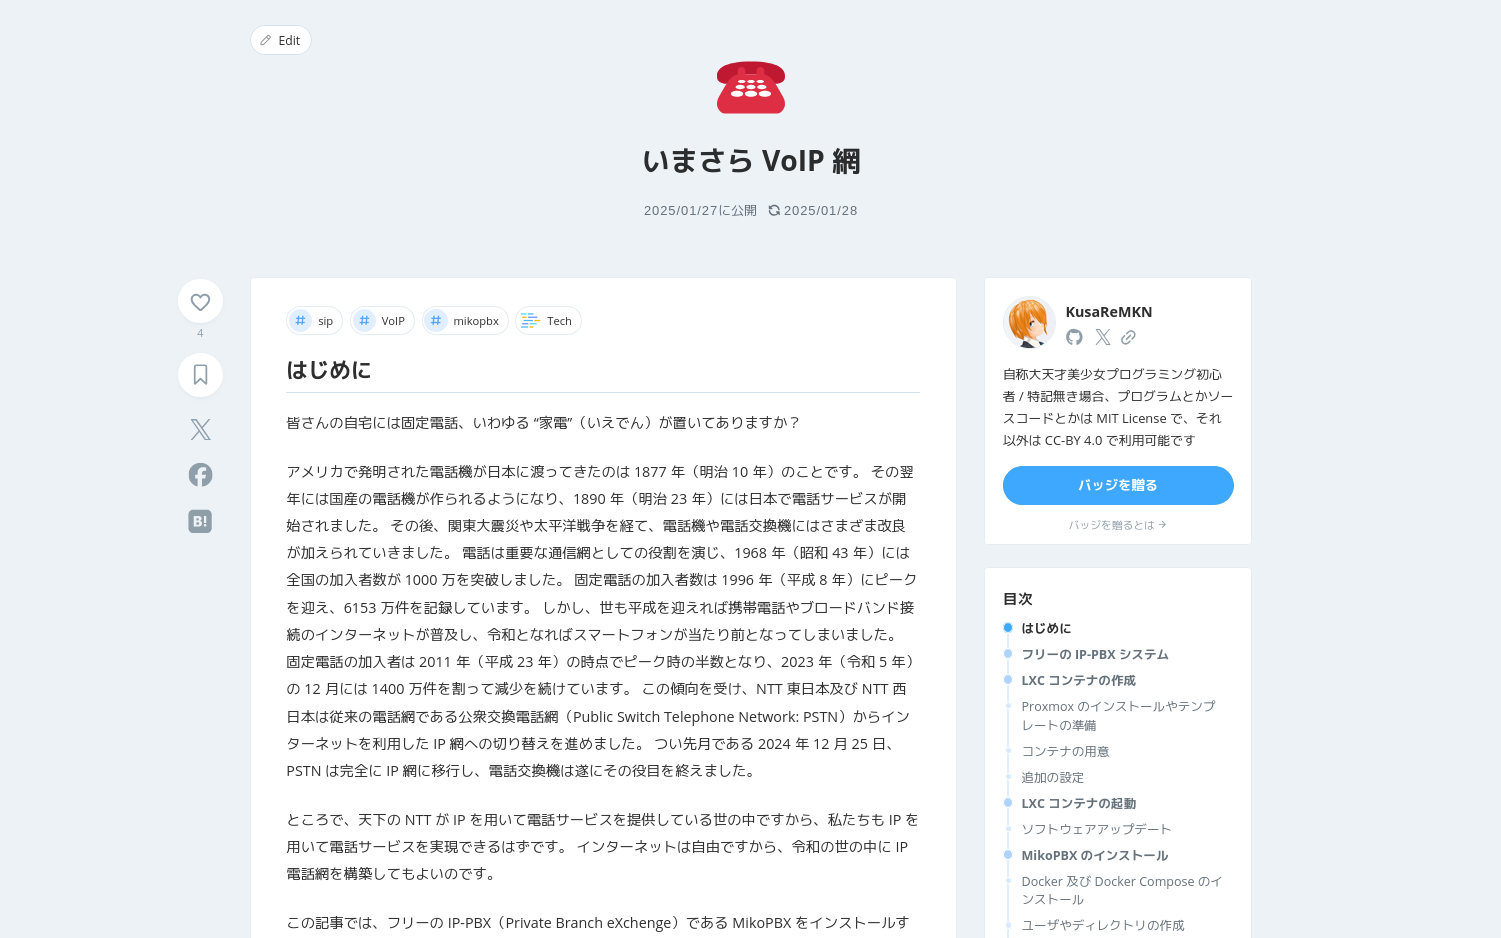
\includegraphics[width=\linewidth]{./images/imasara.png}
\end{frame}

\begin{frame}
  \frametitle{今日のレジュメ(宣伝(1回目))}

  \begin{description}[labelwidth=\linewidth,itemsep=\zh]
    \item[いまさらVoIP網]
      {\small
      \url{https://zenn.dev/kusaremkn/articles/abd760f9f2f450}}
    \item[VoIPルータを使って黒電話をIP電話機にする]
      {\small
      \url{https://zenn.dev/kusaremkn/articles/187222dc1d4f1d}}
    \item[ICOM VE-TA10を使うためにパケットを書き換えたりする]
      {\small
      \url{https://zenn.dev/kusaremkn/articles/cb32b500fc1334}}
  \end{description}
\end{frame}

\section*{みかんちゃんについて}

\begin{frame}
  \frametitle{自称・大天才美少女プログラミング初心者}

  \begin{textblock*}{0.5\paperwidth}(0.6cm, 3.5cm)
    
\includegraphics[width=0.3\paperwidth]{./images/mikanchan.png}
  \end{textblock*}
  \begin{columns}
    \begin{column}{0.30\textwidth}
      \\~\\[-.25\baselineskip]
    \end{column}
    \begin{column}{0.69\textwidth}
      \\~\\[-.25\baselineskip]
      「\ruby{上羽}{うわ|ば} \ruby{未栞}{み|かん}」
      あるいは「\ruby[g]{KusaReMKN}{くされみかん}」\\
      \hspace{1.5\zw}\textbf{みかんちゃん}って呼んでね!
      \\~\\[-.5\baselineskip]

      \newlength{\zeropeke}
      \settowidth{\zeropeke}{\tiny 0x}
      \hspace{-\zeropeke}{\tiny 0x}18\nobreak 歳のJK(重要)
      \\~\\[-.5\baselineskip]

      実はプログラマでもエンジニアでもない\\
      \hspace{1.5\zw}古い計算機っぽいものが大好き
      \\~\\[-.5\baselineskip]

      Twitterで思想を垂れ流すことが得意\\
      \hspace{1.5\zw}\url{https://kusaremkn.com/}も見てね
    \end{column}
  \end{columns}
\end{frame}

\section{「でんわ」のはじまり}

\begin{frame}
  \frametitle{HARD OFFに売られていた黒電話(白色)}

  \centering
  \includegraphics[height=.85\textheight]{./images/ivory.jpeg}
\end{frame}

\begin{frame}
  \frametitle{一方そのころ、限界セルフホスティング界隈では……}

  \begin{columns}[c]
    \begin{column}[c]{.80\textwidth}
      \ruby[g]{\bfseries MMTNET}{ももたねつと}:\\
      \hspace{1.5\zw}Malleable Mutual Tunneling Network\\
      \hspace{1.5\zw}for Experimental Technologies
      \\~\\[-.5\baselineskip]

      SoftEther VPNを使ってホストを相互接続\\
      \hspace{1.5\zw}自作インターネットを目論んでいた
      \\~\\[-.5\baselineskip]

      MMTNET上で動作するアプリケーション\\
      \hspace{1.5\zw}黒電話を利用したIP電話が挙げられていた\\
      \hspace{1.5\zw}MMTNETの前身(HVCAN)でも運用されていた
    \end{column}
    \begin{column}{.17\textwidth}
      \centering
      \\~\\[-.75\baselineskip]
      
\includegraphics[width=\linewidth]{./images/pepepper.jpg}

      
\includegraphics[width=\linewidth]{./images/yude.jpg}

      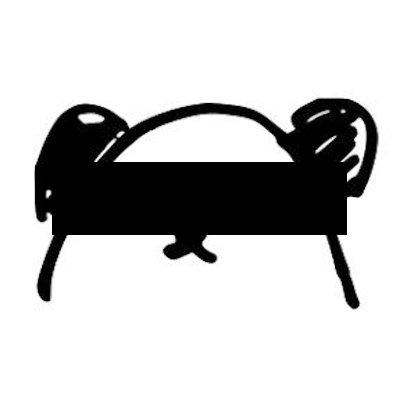
\includegraphics[width=\linewidth]{./images/kurari.jpg}
    \end{column}
  \end{columns}
\end{frame}

\begin{frame}
  \frametitle{HVCAN上のIP電話発足の貴重なシーン}

  ~\\[-.75\baselineskip]
  \begin{columns}[b]
    \begin{column}{.49\textwidth}
      \centering
      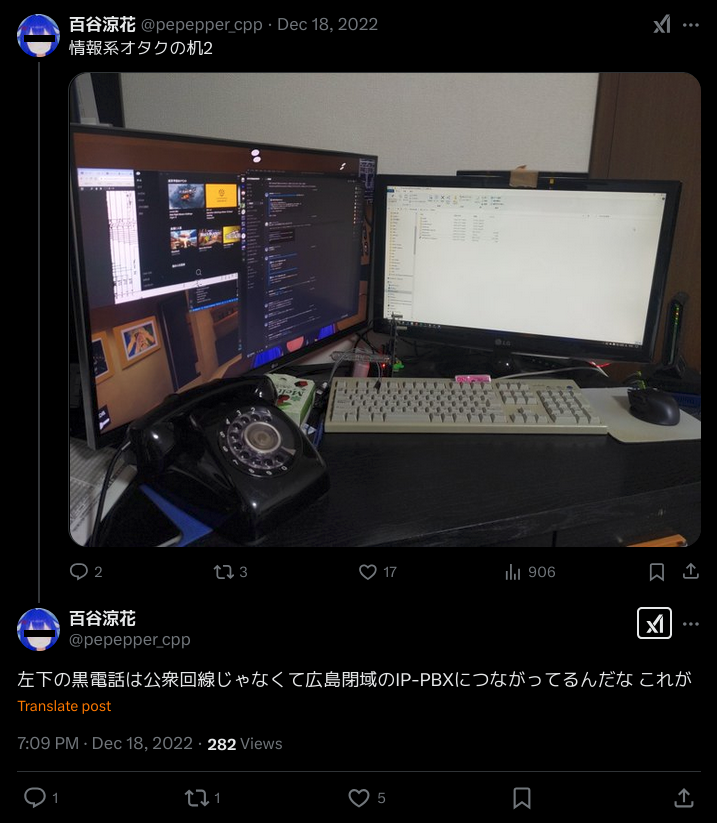
\includegraphics[height=.9\textheight]{./images/ijyou.png}
    \end{column}
    \begin{column}{.49\textwidth}
      \centering
      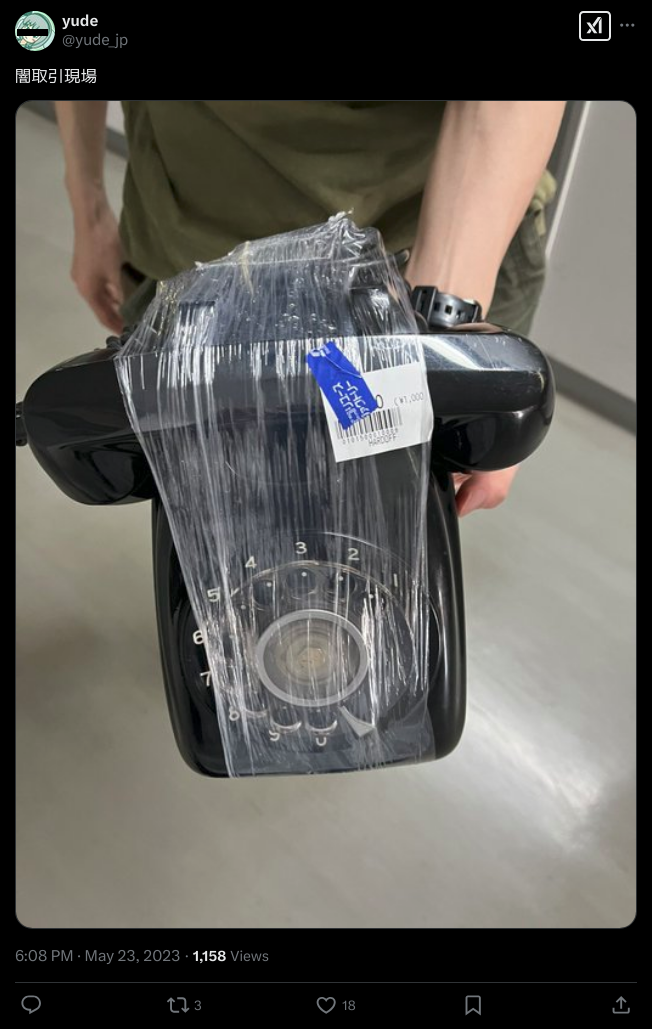
\includegraphics[height=.9\textheight]{./images/yami.png}
    \end{column}
  \end{columns}
  \centering
\end{frame}


\begin{frame}
  \frametitle{HVCAN上の電話網(?)の様子}

  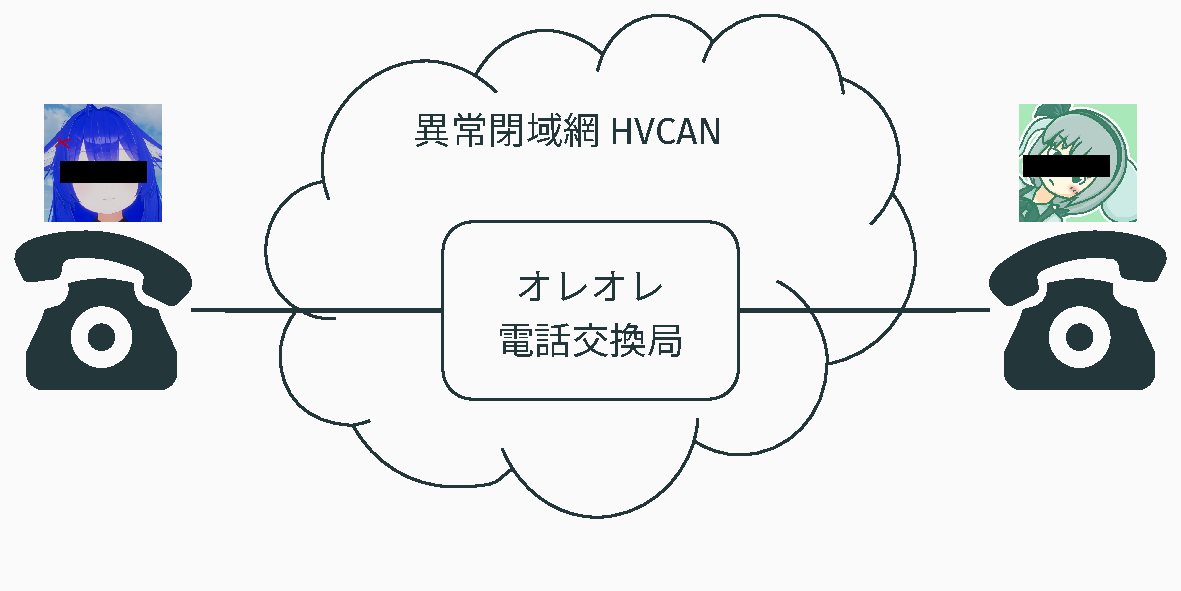
\includegraphics[page=1,width=\linewidth]{./images/pictures.pdf}
\end{frame}

\begin{frame}
  \frametitle{実現したいこと}

  \begin{description}[labelwidth=\linewidth,itemsep=.25\zh]
    \item[外線通話と多局接続]
      交換局をまたぐ通話\\
      複数の交換局の相互接続
    \item[交換局ホップ]
      相互接続されていない局の通話
  \end{description}

  状況を簡単にするためMMTNETから切り離される\\
  \hspace{1.5\zw}オレオレ電話網「\textbf{東京広域電話網}」の爆誕
\end{frame}

\section{外線通話と多局接続}

\begin{frame}
  \frametitle{基本の構成}

  \begin{columns}
    \begin{column}{.6\textwidth}
      交換局として\textbf{MikoPBX}を用いる\\
      \hspace{1.5\zw}AsteriskベースのIP-PBXシステム\\
      \hspace{1.5\zw}シンプルなWEB UIが魅力
      \\~\\[-.5\baselineskip]

      スタンドアロン版とDocker版がある
    \end{column}
    \begin{column}{.39\textwidth}
      
\includegraphics[width=\linewidth]{./images/mikopbx.png}
    \end{column}
  \end{columns}
\end{frame}

\begin{frame}
  \frametitle{ダメなシステム構成(その1)}

  \includegraphics[page=2,width=\linewidth]{./images/pictures.pdf}
\end{frame}

\begin{frame}
  \frametitle{VPNを使えばいいじゃない}

  \begin{columns}
    \begin{column}{.6\textwidth}
      交換局間の接続に\textbf{Tailscale}を用いる\\
      \hspace{1.5\zw}簡単なメッシュ型VPNサービス\\
      \hspace{1.5\zw}ユーザ間で接続を共有できてお得
    \end{column}
    \begin{column}{.39\textwidth}
      
\includegraphics[width=\linewidth]{./images/tailscale.png}
    \end{column}
  \end{columns}
\end{frame}

\begin{frame}
  \frametitle{ダメなシステム構成(その2)}

  \includegraphics[page=3,width=\linewidth]{./images/pictures.pdf}
\end{frame}

\begin{frame}
  \frametitle{Docker版を使えばいいじゃない}

  \begin{columns}
    \begin{column}{.6\textwidth}
      \textbf{Docker}版MikoPBXを用いる\\
      \hspace{1.5\zw}ホスト側でTailnetに接続\\
      \hspace{1.5\zw}MikoPBX側は何も考えなくてよい
    \end{column}
    \begin{column}{.39\textwidth}
      
\includegraphics[width=\linewidth]{./images/docker.png}
    \end{column}
  \end{columns}
\end{frame}

\begin{frame}
  \frametitle{完成版のシステム構成}

  MikoPBXの設定をこねくり回していたら外線通話が可能に!

  \includegraphics[page=4,width=\linewidth]{./images/pictures.pdf}

  % これ、2024-11-11 の話かも
\end{frame}

\begin{frame}
  \frametitle{多局接続がむつかしい}

  \includegraphics[page=5,width=\linewidth]{./images/pictures.pdf}
\end{frame}

\begin{frame}
  \frametitle{WEBに表示されていない設定項目}

  % 2024-11-23
  \begin{columns}
    \begin{column}{.7\textwidth}
      MikoPBXのWEB UIで設定を変更すると\\
      \hspace{1.5\zw}システムの設定ファイルが書き変わる
      \\~\\[-.5\baselineskip]

      WEB UIに表示されていない項目もある\\
      \hspace{1.5\zw}設定項目\texttt{max\_contacts}\\
      \hspace{1.5\zw}デフォルトの値は\textbf{1}\\
      \hspace{1.5\zw}これを100にすると接続できる
    \end{column}
    \begin{column}{.29\textwidth}
      
\includegraphics[width=\linewidth]{./images/jiminy.jpg}
    \end{column}
  \end{columns}
\end{frame}

\section{交換局ホップ}

\begin{frame}
  \frametitle{新しい局を追加する際の手間}

  \includegraphics[page=6,width=\linewidth]{./images/pictures.pdf}
\end{frame}

\begin{frame}
  \frametitle{インターネットにできるなら電話網にもできる}

  インターネットのルータは完全グラフを構成していない\\
  \hspace{1.5\zw}それでも多くのホストと通信できる
  \\~\\[-.5\baselineskip]

  電話網の全ての局が完全グラフを構成していない場合\\
  \hspace{1.5\zw}局同士がよしなに通話を取り持ってくれれば\\
  \hspace{1.5\zw}直接接続されていない局間でも通話を実現できるのでは?
\end{frame}

\begin{frame}
  \frametitle{電話を掛け直す電話番号}

  % 2024-11-23
  \begin{columns}
    \begin{column}{.7\textwidth}
      通常の外線着信の場合\\
      \hspace{1.5\zw}\textbf{着信局内の端末のみ}を対象に検索\\
      \hspace{1.5\zw}→ 再び\textbf{外線接続することはない}
      \\~\\[-.5\baselineskip]

      特定の番号に電話を掛けた場合\\
      \hspace{1.5\zw}番号を検索する部分でインチキをする\\
      \hspace{1.5\zw}\textbf{外線の番号}も検索しなおしてもらう\\
      \hspace{1.5\zw}→ 再び\textbf{外線接続のチャンスがやってくる}
    \end{column}
    \begin{column}{.29\textwidth}
      
\includegraphics[width=\linewidth]{./images/jiminy.jpg}
    \end{column}
  \end{columns}
\end{frame}

\begin{frame}
  \frametitle{相互接続されていない局間でも通話が可能に}

  \includegraphics[page=7,width=\linewidth]{./images/pictures.pdf}
\end{frame}

\section{実際に運用してみた結果}

\begin{frame}
  \frametitle{実験と運用の日々}

  「\textbf{東京広域電話網}」のプロジェクト開始が2024年10月中旬
  \\~\\[-.5\baselineskip]

  現在(2025年2月)に至るまで約4ヶ月間ほど実運用\\
  \hspace{1.5\zw}Webから通話できるアプリケーションの実現\\
  \hspace{1.5\zw}時報やモーニングコールなどのサービスも実現\\
  \hspace{1.5\zw}電話だけでなくFAXやダイヤルアップ通信も動作確認
  \\~\\[-.5\baselineskip]

  電話網の相互接続状況を記述するJSON Schemaを開発\\
  \hspace{1.5\zw}\url{https://github.com/KusaReMKN/mantela}\\
  \hspace{1.5\zw}\url{https://github.com/KusaReMKN/mantela-viewer}
\end{frame}

\begin{frame}
  \frametitle{現在の東京広域電話網の姿}

  \begin{columns}
    \begin{column}{.25\textwidth}
      \begin{description}[labelwidth=\linewidth]
        \item[交換局数]
          13局
        \item[端末数]
          58以上\\
          (仮想含む)
        \item[うち黒電話]
          10程度
        \item[その他]
          公衆電話\\
          ワープロ
      \end{description}
    \end{column}
    \begin{column}{.7\textwidth}
      \centering
      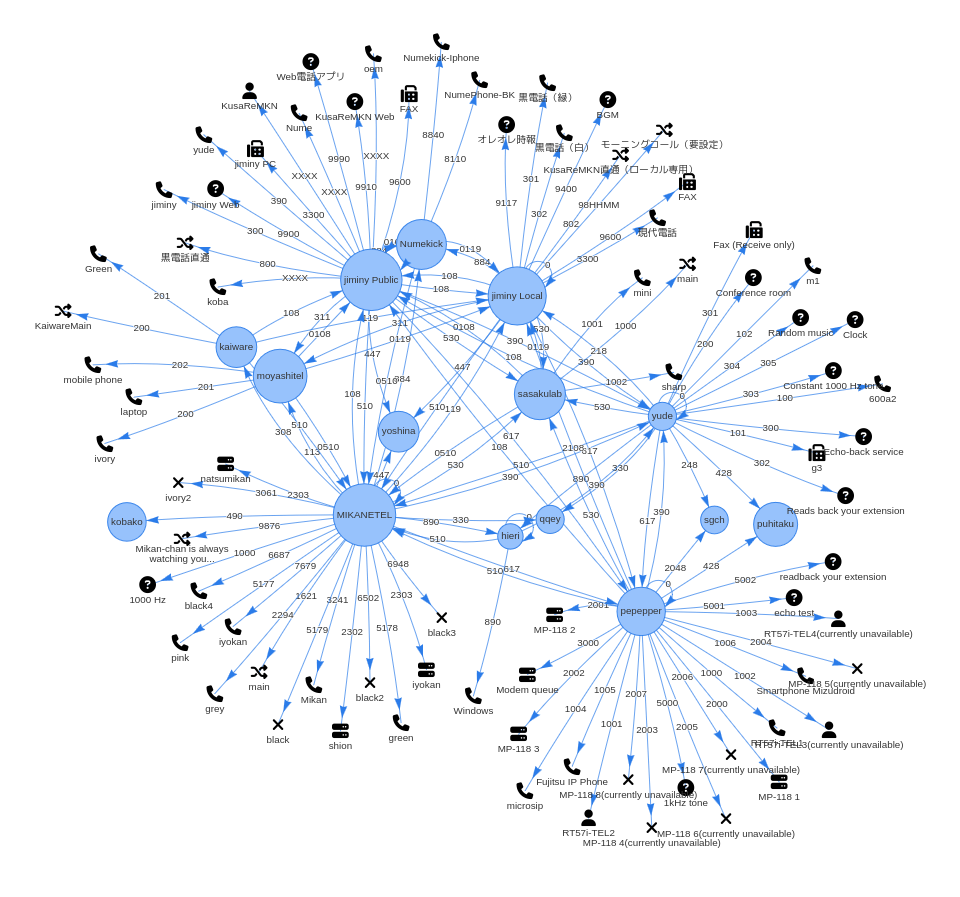
\includegraphics[height=.87\textheight]{./images/mantela.png}
    \end{column}
  \end{columns}
\end{frame}

\begin{frame}
  \frametitle{現在の東京広域電話網の姿}

  \begin{columns}
    \begin{column}{.25\textwidth}
      \begin{description}[labelwidth=\linewidth]
        \item[交換局数]
          13局
        \item[端末数]
          58以上\\
          (仮想含む)
        \item[うち黒電話]
          10程度
        \item[その他]
          公衆電話\\
          ワープロ
      \end{description}
    \end{column}
    \begin{column}{.7\textwidth}
      \centering
      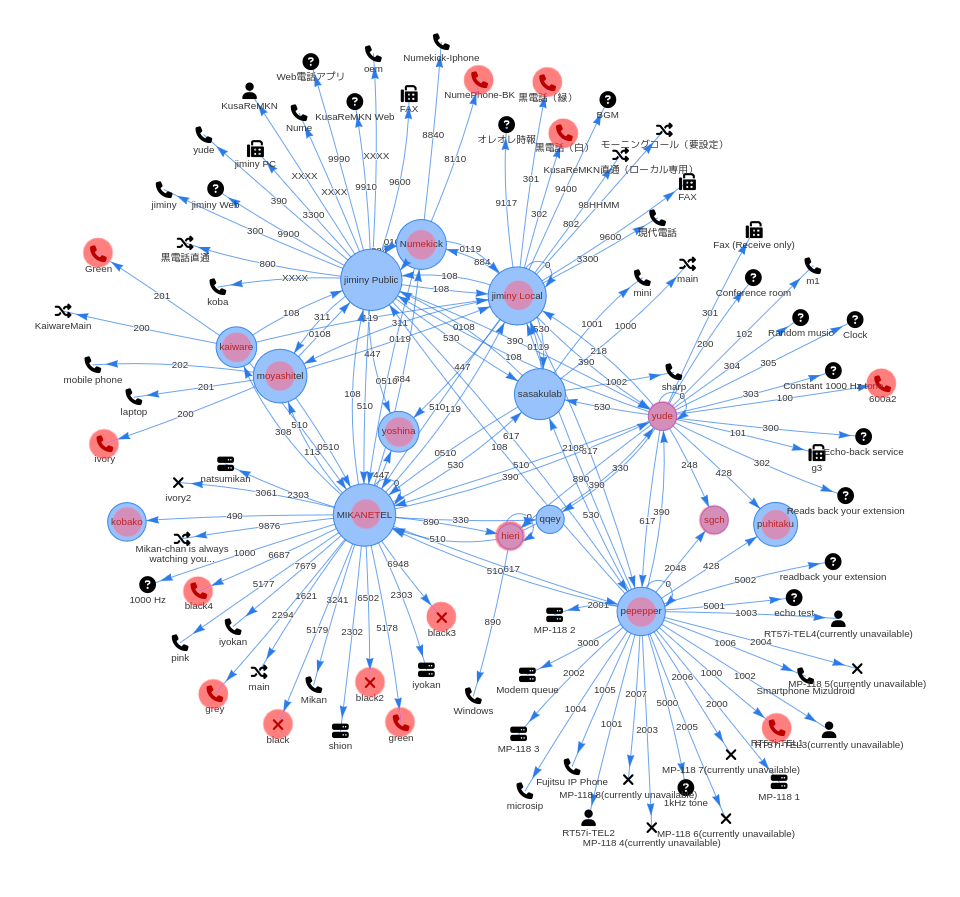
\includegraphics[height=.87\textheight]{./images/mantela2.png}
    \end{column}
  \end{columns}
\end{frame}

\section{みんなも「でんわ」をしよう!}

\begin{frame}
  \frametitle{用意するもの}

  必須なものは\textbf{コンピュータだけ}\\
  \hspace{1.5\zw}交換局を設置・相互接続するだけでOK
  \\~\\[-.5\baselineskip]

  黒電話やFAXなど物理的な端末をぶら下げたい場合は……

  \begin{description}[labelwidth=\linewidth]
    \item[VoIPルータ(ゲートウェイ?)]
      IP通信を電話信号に変換する人\\
      YAMAHA RT57iやRT58iなどで動作確認済\\
      ICOM VE-TA10もインチキすれば動作可能
    \item[端末それ自体]
      電話線の刺さるものはだいたい友達
  \end{description}
\end{frame}

\begin{frame}
  \frametitle{今日のお話の記事(宣伝(2回目))}

  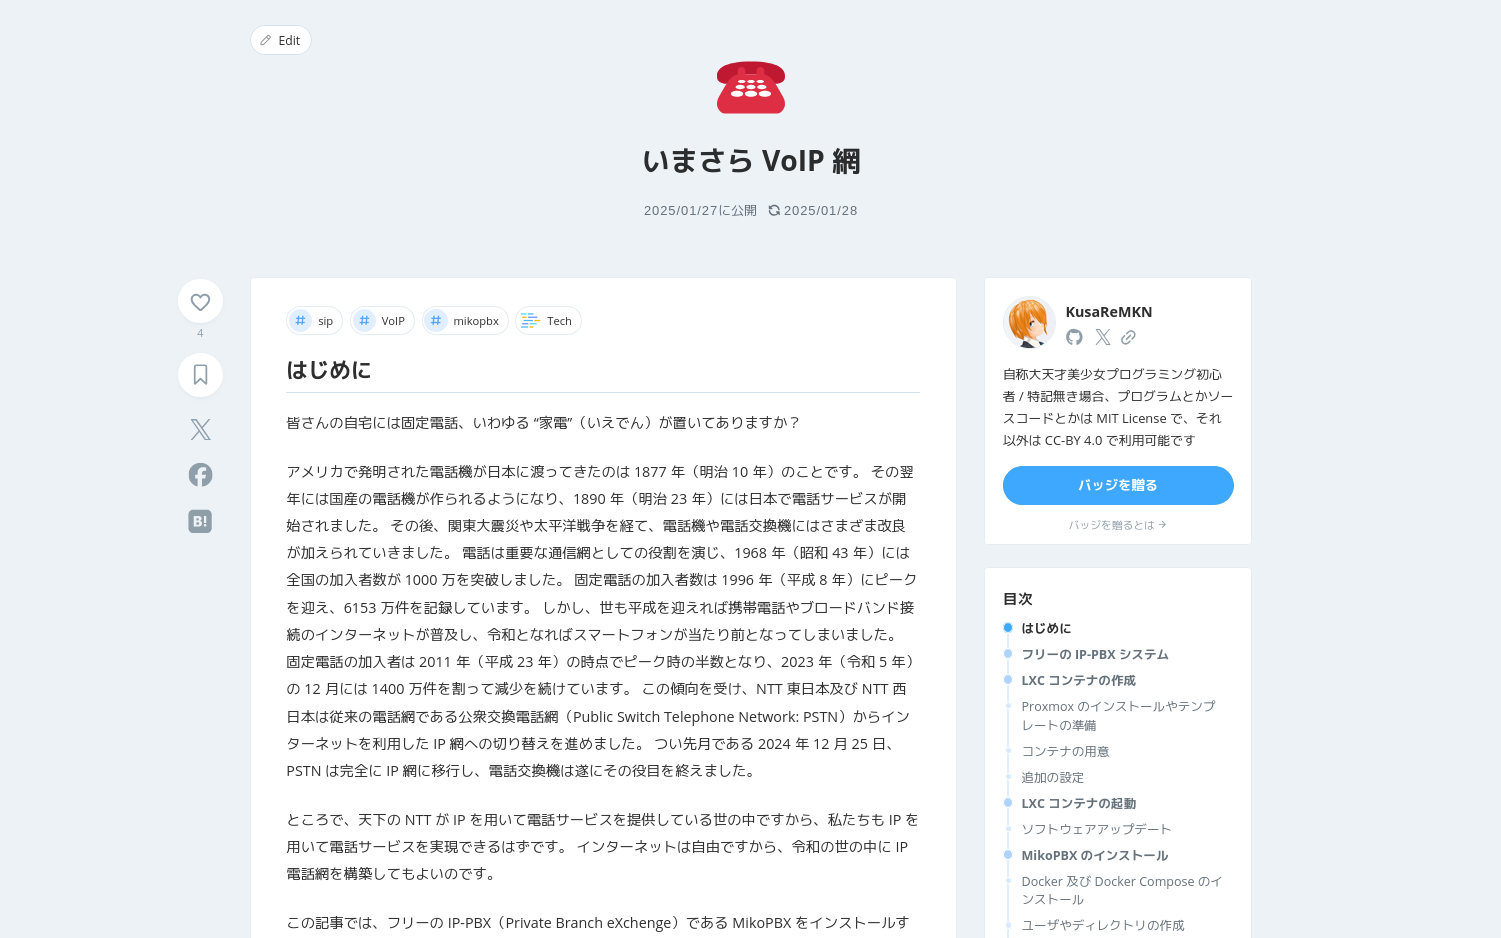
\includegraphics[width=\linewidth]{./images/imasara.png}
\end{frame}

\begin{frame}
  \frametitle{今日のお話の記事(宣伝(2回目))}

  \begin{description}[labelwidth=\linewidth,itemsep=\zh]
    \item[いまさらVoIP網]
      {\small
      \url{https://zenn.dev/kusaremkn/articles/abd760f9f2f450}}
    \item[VoIPルータを使って黒電話をIP電話機にする]
      {\small
      \url{https://zenn.dev/kusaremkn/articles/187222dc1d4f1d}}
    \item[ICOM VE-TA10を使うためにパケットを書き換えたりする]
      {\small
      \url{https://zenn.dev/kusaremkn/articles/cb32b500fc1334}}
  \end{description}
\end{frame}


\section{まとめ}

\begin{frame}
  \frametitle{オレオレIP電話網と黒電話で遊んでみた}

  IP-PBXシステムを利用したIP電話網を構築

  交換局同士の相互接続・多局接続を実現

  交換局ホップの実現(相互接続されていない局間での通話)

  今後は電話網上のアプリケーションについて報告できたらいいな
\end{frame}

\begin{frame}[standout]
  おわりです
\end{frame}

\begin{frame}
  \frametitle{このスライドについて}

  Written in February 2025.\\
  \hspace{1.5\zw}Permanent ID of this document: \texttt{55b54dae70afe9e9}.
  \\~\\[-.5\baselineskip]

  Copyright © 2025 KusaReMKN.
  \\~\\[-.5\baselineskip]

  特記無き場合、プログラムやソースコードは MIT License で、\\
  \hspace{1.5\zw}それ以外のコンテンツは CC-BY 4.0 で利用可能です。\\
  \hspace{1.5\zw}一部の画像には別のライセンスが適用されるかもしれません。
\end{frame}

\end{document}
% ex: se et ts=2 :
